\chapter{Open Research Directions} \label{Chap:Bench}




\section{Benchmarking of Task-based Heterogeneous Applications}

\lettrine[findent=2pt]{\textbf{T}}{}he benchmark is composed of six parallel applications. Five of them have been generated from Chameleon, a dense linear algebra software which is part of the MORSE project~\cite{agullo2012morse}, while the sixth has been generated with GGen, a library for generating directed acyclic graphs~\cite{GGen:simutools10}, and it corresponds to a more irregular application.


\subsection{Chameleon Benchmark}
This benchmark have been generated for the purpose of two scientific papers:
\begin{itemize}
 \bibitem[Mommessin {\rm{\em et~al.}} (2017)Mommessin, Amaris, Lucarelli, e
  Trystram]{Mommessin:2017}
Clement~Mommessin, {\bf Marcos~Amaris}, Giorgio~Lucarelli and Denis~Trystram.
\newblock Generic algorithms for scheduling applications on hybrid multi-core
  machines.
\newblock In \emph{2017 Euro-Par: International Conference on Parallel and
  Distributed Computing}, pages 220--231. 
  
  \bibitem[Mommessin {\rm{\em et~al.}} (2018)Mommessin, Amaris, Lucarelli, e
  Trystram]{mommesin:2017:CCPE}
Clement~Mommessin, {\bf Marcos~Amaris}, Giorgio~Lucarelli and Denis~Trystram.
\newblock Generic algorithms for scheduling applications on heterogeneous multi-core platforms
\newblock \emph{arXiv preprint arXiv:1711.06433} in revision. Submmited in 
\emph{Concurrency and Computation: Practice and Experience}
\end{itemize} 

Five applications were chosen of Chameleon software to create this benchmark, these are  \texttt{getrf\_nopiv}, \texttt{posv}, \texttt{potrs}, \texttt{potri} and \texttt{potrf}, these aplication are composed of multiple sequential basic tasks of linear algebra. Task or kernels among are \texttt{SYRK} (symetric rank update), \texttt{GEMM} (general matrix-matrix multiply) and \texttt{TRSM} (triangular matrix equation solver), among other. Figure~\ref{fig:DAGspotrf} shows the DAG of the application Cholesky Factorization, which is the application \texttt{potrf}. For both workloads with 2 and 3 resource types the Chameleon applications were executed with the runtime StarPU~\citep{agullo2012morse} and the traces of executions were collected. 

At first, all the applications were executed on CPUs and then were forced to execute on GPUs to have the processing times of each task of the application for different resources.


The five applications of Chameleon, named \emph{getrf$\_$nopiv}, \emph{posv}, \emph{potrs}, \emph{potri} and \emph{potrs}, are composed of multiple sequential basic tasks of linear algebra such as \emph{SYRK} (symetric rank update), \emph{GEMM} (general matrix-matrix multiply) and \emph{TRSM} (triangular matrix equation solver), as shown in Table~\ref{tab:kernels}. 



\begin{figure}[htpb]
	\centering
    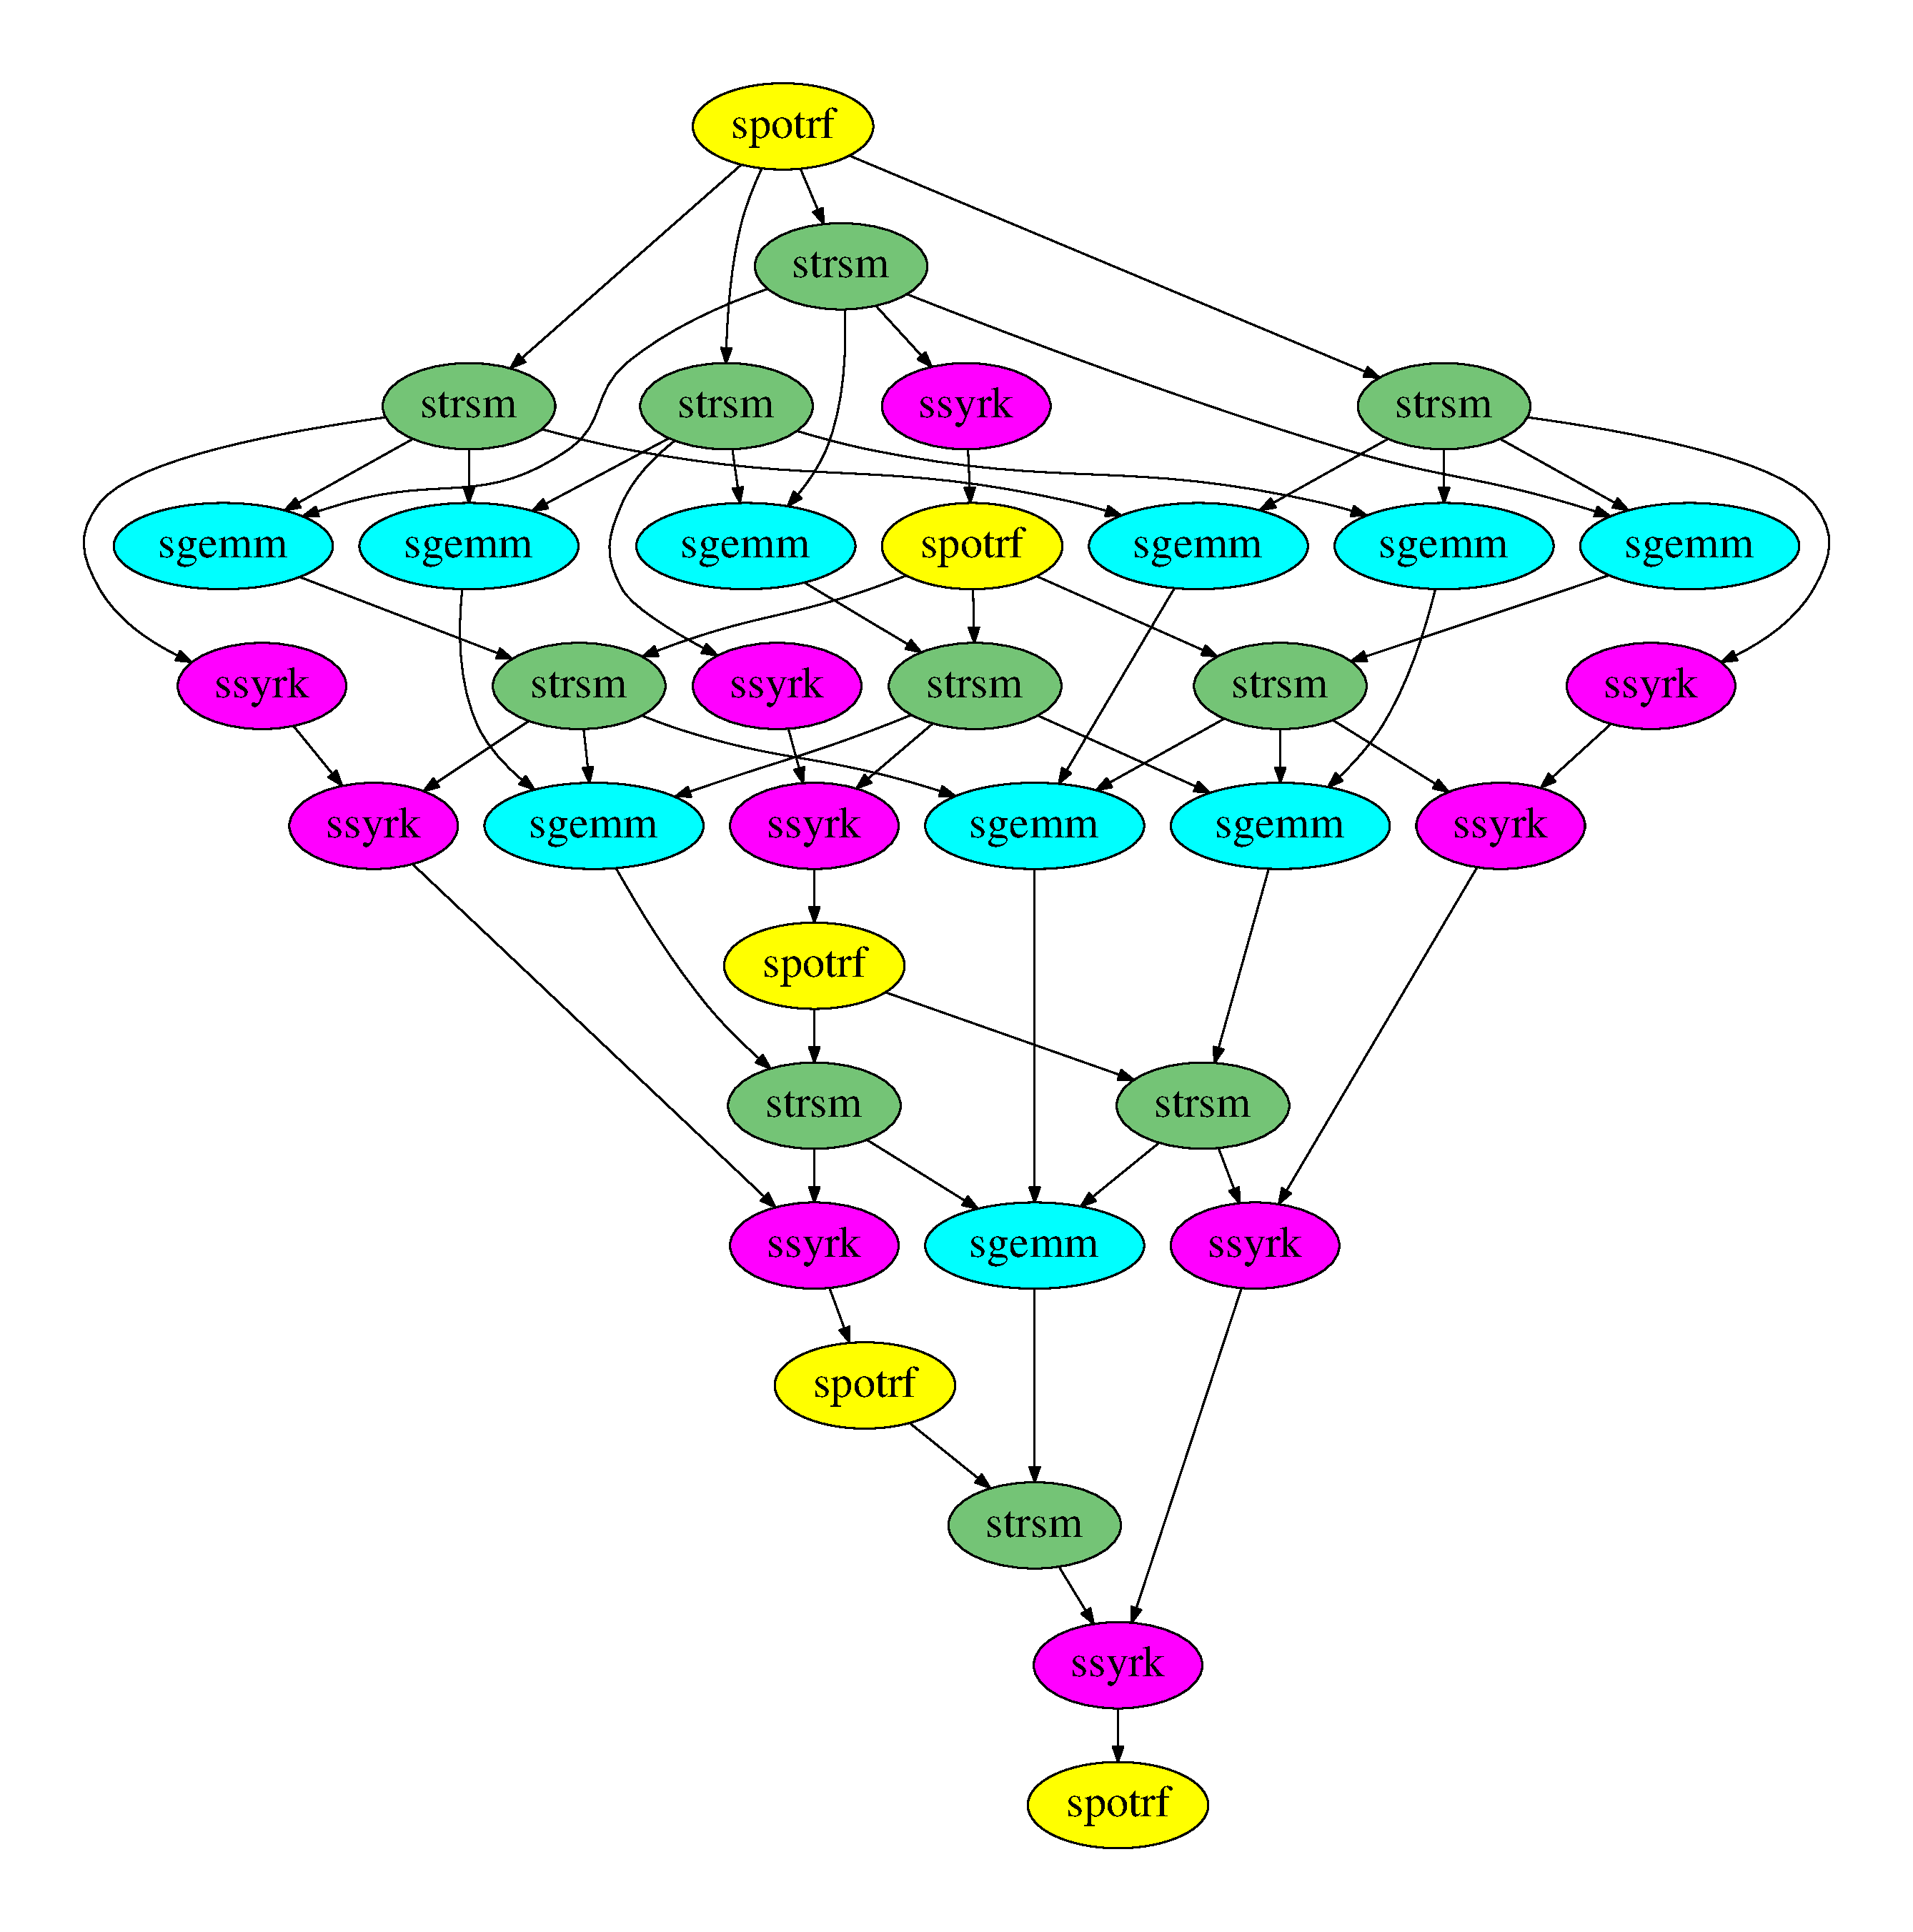
\includegraphics[scale=.3]{images/DAGspotrf.pdf}
    \caption{DAGspotrf}
    \label{fig:DAGspotrf}
\end{figure}


\begin{table}[htpb]
\begin{center}
\begin{tabular}{|c|c|c|c|c|c|c|}
	\hline
	\backslashbox{\bf Kernels}{\bf Apps} & {\bf getrf$\_$nopiv} & {\bf posv} & {\bf potrf} & {\bf potri} & {\bf potrs}\\
	\hline
	{\bf syrk}& & x & x & x & \\
	\hline
	{\bf gemm}& x & x & x & x & x \\
	\hline
	{\bf trsm}& x & x & x & x & x \\
	\hline
\end{tabular}
\caption{Basic kernel of linear algebra of each application}
\label{tab:kernels}
\end{center}
\end{table}

To generate the applications, different tilings of the matrices have been used, varying the number of sub-matrices denoted by $nb\_blocks$ and the size of the sub-matrices denoted by $block\_size$. The different values of $nb\_blocks$ were 5, 10 and 20 and the different values of $block\_size$ were 64, 128, 320, 512, 768 and 960, for a total of 18 configurations per application. Table \ref{fig:nb_tasks} shows the total number of tasks for each application and each value of $nb\_blocks$. Notice that the value of $block\_size$ does not impact the number of tasks.

\begin{table}[htpb]
\begin{center}
\begin{tabular}{|c|c|c|c|c|c|c|}
	\hline
	\backslashbox{\bf Nb$\_$blocks}{\bf Apps} & {\bf getrf$\_$nopiv} & {\bf posv} & {\bf potrf} & {\bf potri} & {\bf potrs} \\
	\hline
	{\bf 5} & 55 & 65 & 35 & 105 & 30 \\
	\hline
	{\bf 10} & 385 & 330 & 220 & 660 & 110 \\
	\hline
	{\bf 20} & 2870 & 1960 & 1540 & 4620 & 420 \\
	\hline
\end{tabular}
\caption{Total number of tasks in function of the number of blocks}
\label{fig:nb_tasks}
\end{center}
\end{table}
The Chameleon applications were executed with the runtime StarPU~\cite{Augonnet:StarPU} and the traces of executions were collected. At first, all the applications were executed on CPUs and then were forced to execute on GPUs to have the processing times of each task of the application for both computing units.

The machine where this data was collected had the following hardware characteristics: Dual core Xeon E7 v2, with a total of 20 physical cores  with hyper-threading of 3 GHz of processor base Frequency, 256 GB of RAM, operative system Linux Ubuntu 14.04. This machine had 4 GPUs NVIDIA Tesla K20 with each 4 GB of global memory, 200 GB/s of bandwidth and 2496 cores divided in 13 multiprocessors.

%The SWF was defined in order to ease the use of workload logs and models. With it, programs that analyze workloads or simulate system scheduling need only to be able to parse a single format, and can be applied to multiple workloads. 
% The data set and other information are available\footnote{Hosted at: \url{https://github.com/marcosamaris/heterogeneous-SWF} [Accessed on 19 October 2016]} under Creative Commons Public License for the sake of reproducibility.

\subsection{Fork-joint Benchmark}
The application generated with GGen is \emph{fork-join}. It represents a real application that starts by executing sequentially and then forks to be executed in parallel with a specific diameter (number of parallel tasks), when the parallel execution has completed, results are aggregated by performing a join operation. This procedure can be repeated several times depending on the number of phases. For our experiments, we used 2, 5 and 10 phases with a diameter of 100, 200, 300, 400 and 500 for a total of 15 different configurations. Table \ref{fig:nb_tasksFork} shows the total number of tasks for each configuration of the fork-join application.

\begin{figure}[htpb]
	\centering
    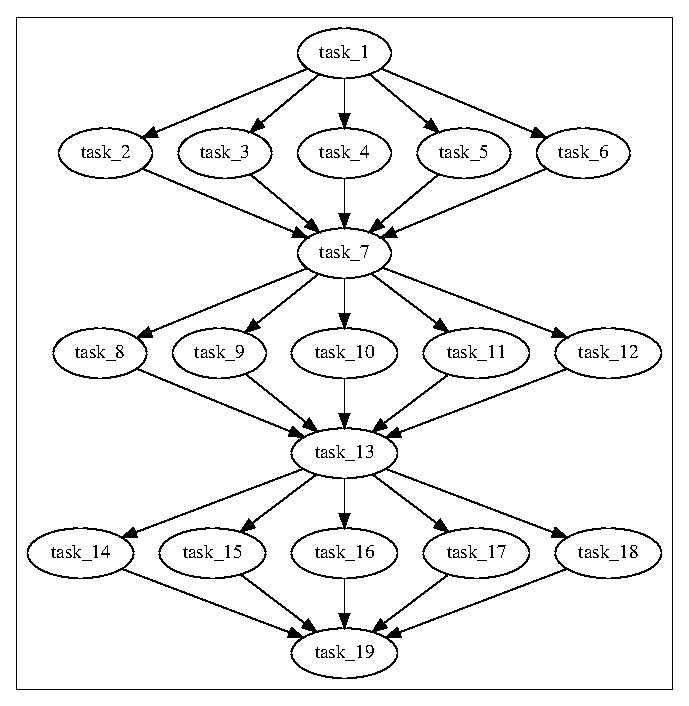
\includegraphics[scale=.5]{images/forkjoin-3-5.png}
    \caption{Fork-join application with 3 phases and 5 parallel and concurrent tasks}
    \label{fig:forkjoin}
\end{figure}



\begin{table}[htpb]
\begin{center}
\begin{tabular}{|c|c|c|c|c|c|c|}
	\hline
	\backslashbox{\bf Nb$\_$phases}{\bf Diameter} & {\bf 100} & {\bf 200} & {\bf 300} & {\bf 400} & {\bf 500} \\
	\hline
	{\bf 2} & 203 & 403 & 603 & 803 & 1003 \\
	\hline
	{\bf 5} & 506 & 1006 & 1506 & 2006 & 2506 \\
	\hline
	{\bf 10} & 1011 & 2011 & 3011 & 4011 & 5011 \\
	\hline
\end{tabular}
\caption{Total number of tasks in function of the number of phases and the width of the phase}
\label{fig:nb_tasksFork}
\end{center}
\end{table}
The running time of each task was computed using a Gaussian distribution with center $p$ and standard deviation $\frac{p}{4}$, where $p$ is the number of phases. We have decided to establish various acceleration factors in each diameter of fork. In this way, for all the configurations there are five parallel tasks with an acceleration factor between $0.1$ and $0.5$ while the others have an acceleration factor between $0.5$ and $50$.

% \subsection{SWF e Dependencies Files}
The execution time of each task and their respective dependencies were collected and formatted in different files, in SWF~(Standard Workload Format). The SWF standard was defined in order to ease the use of workload logs and models. With it, programs that analyze workloads or simulate systems scheduling need only to be able to parse a single format, and can be applied to multiple workloads.

% \subsection{Online Scheduling Techniques}


\section{Performance Predictions on Hybrid CPU-GPU 2D Stencil 5-point Application}

\subsection{Concurrent Streams on GPU}\label{sec:StreamGPU}
Heterogeneous computing is about efficiently using all processors in the system, including CPUs and GPUs.  In our heterogeneous systems, GPUs have been connected to a host machine by a high bandwidth interconnect such as PCI Express (PCIe). Host and device have different memory address spaces, and data must be copied back and forth between the two memory pools explicitly by the data transfer functions. 
%There are two main aspects to consider when attempting to run an application on both CPUs and GPUs concurrently, namely the communication costs incurred by CPU-GPU communications, and how to efficiently overlap computation and data transfers to reduce said cost.
%On integrated CPU/GPU architectures, ~\cite{Zhang17} suggested that the architecture differences between CPUs and GPUs, as well as limited shared memory bandwidth, are two main factors affecting co-running performance. 
%On SMP systems connected to GPU architectures, beside architectural differences, communications between CPUs and GPUs are another important factor. 
Servers with multi-cores and multi-accelerator devices are primarily connected by PCI-Express (PCIe) bus. GPUs and CPUs are bridged by a PCIe bus. Data are copied from the CPU host memory to PCIe memory first, and are then transferred to the GPU's global memory. The PCIe bandwidth is always a crucial performance bottleneck to be improved. 

Congestion control mechanisms have a significant impact on communications. Moreover, the PCIe congestion behavior varies significantly depending on the conflicts created by communication. \cite{Martinasso16} have explored the impact of PCIe topology, which is one major parameter influencing the available bandwidth. They developed a congestion-aware performance model for PCIe communication. They found that bandwidth distribution behavior is sensitive to the transfer message size. PCIe congestion can be hidden if the overlapping communications transfer very small message sizes. However, when the message size reaches some limit, congestion will significantly reduce the theoretical transfer bandwidth efficiency and the bandwidth between the CPU host memory and the GPU memory is far less than PCIe bandwidth. Nvidia provides ways to pin memory, also called paged-locked memory~\citep{CUDAGuide}. A pinned page can be remapped to a PCIe buffer to eliminate data transfer between the host memory and the PCIe buffer. However, consuming too much page-locked memory will reduces overall system performance.

CUDA's programming model provides constructs based on streaming which are capable to schedule multiple kernels concurrently. One CUDA stream can encapsulate multiple kernels, and they have to be scheduled so they strictly follow a particular order. However, kernels from multiple streams can be scheduled to run concurrently. Operations in different streams can be interleaved and overlapped, which can be used to hide data transfers between host and device.

A optimization of GPU applications is to overlap data transfers across the PCIe bus~\citep{Martinasso16}. This is only possible using CUDA streams and pinned memory in the host. Using pinned host memory enables asynchronous memory copies, lowers latency, and increases bandwidth. This way, streams can run concurrently. However, this goal is constrained by the number of kernel engines and copy engines exposed by GPUs, and synchronization must be explicit in the stream kernels. In order to obtain the best performance, a balance between computation and communication needs to be found. If the granularity is too fine, the performance can suffer from the increased communication overhead. On the other side, if the granularity is too coarse or bulk, the performance can suffer from load imbalance. 

There are GPUs with only a single copy engine and a single kernel engine. In this case, data transfer overlapping is not possible. Different streams may execute their commands concurrently or out of order with respect to each other. When an asynchronous CUDA stream is executed without specifying a stream, the CUDA runtime uses the default stream 0; but when a set of independent streams are executed with different ID numbers, these streams avoid serialization, achieving concurrency between kernels and data copies.

Figure~\ref{fig:streams} explains how the streaming model is used to improve the performance of GPU applications. In this figure, we compare the parallel CPU computations of two different GPU version with their respective data transfers: one single stream vs. 3 different kernels with their respective data transfers using 3 streams. The second method is only possible in GPUs with two copy engines, one for host-to-device transfers and another for device-to-host transfers. 


\begin{figure}
	\centering
%     \includegraphics[width=\linewidth]{fig/streams}
    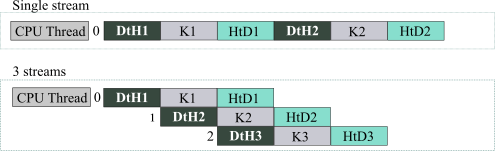
\includegraphics[scale=.8]{images/stream.png}
    \caption{Concurrent Streams overlapping data transfers}
    \label{fig:streams}
%\vspace{-15pt}
\end{figure}











